
\documentclass{beamer}
\usepackage[utf8]{inputenc}
\usepackage[ngerman]{babel}
\usepackage{multicol}
\usepackage[utf8]{inputenc}
\usepackage[T1]{fontenc}
\usepackage[ngerman]{babel}
\usepackage{amsmath}
\usepackage{amsfonts}
\usepackage{amssymb}
%\usepackage{paralist}
\usepackage{color}
\usepackage{xcolor}
\usepackage{lmodern}
\usepackage{graphicx}
\usepackage[mediumspace,mediumqspace,squaren]{SIunits} %SI-Einheiten
\usepackage[version=3]{mhchem} %chemische Formeln
\usepackage{tabularx, calc} %Tabellen
\usepackage{multirow} %Tabelle: mehrere Spalten vereinigen
\usepackage{booktabs} %Verbesserung der Tabellenqualität
\usepackage{caption} %Abbildungs- und Tabellenbeschriftung
\usepackage{array} %Matheumgebung ähnlich tabular
\usepackage{pgf}
\usepackage{dcolumn}
\usepackage{beamerthemeshadow}
\usepackage{comment}
\usepackage{framed}
\usepackage{longtable}
 \usepackage{arydshln}
\beamersetuncovermixins{\opaqueness<1>{25}}{\opaqueness<2->{15}}
\begin{document}
\title{Bachelorarbeit}
\subtitle{Disambiguierungsstrategien in Dialogsystemen }  
%\title{Disambiguierungsstrategien in Dialogsystemen }
%\subtitle{Bachelorarbeit}
\author{Lena Enzweiler}
\institute{Universität des Saarlandes}
\date{\today} 

\beamertemplatenavigationsymbolsempty

\setbeamertemplate{footline}[frame number]

\frame{\titlepage} 

\section{Einleitung}

\subsection{Dialogsystem in automobilen Anwendungen}
\frame{\frametitle{Dialogsystem in automobilen Anwendungen}
Effiziente Dialogsysteme im Auto müssen folgende Punkte erfüllen
\begin{figure}[h]
%\caption{Funktionsweise der odp-s3 Platform der Semvox GmbH}
	%\centering
        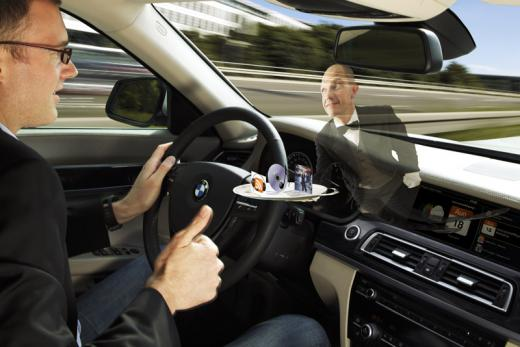
\includegraphics[scale=0.26]{incarassi}
\end{figure}
\begin{itemize}
\item Ablenkung während der Fahrt vermeiden
\item alle Informationen kurz und verständlich übermitteln
\item einfache und intuitive Bedienung garantieren 
\end{itemize} 

$\rightarrow$ Sprachäußerungen müssen durchdacht gestaltet werden
}
\subsection{Fokus der Studie}
\frame{\frametitle{Fokus der Studie}
\begin{figure}[htbp]
	% minipage mit (Blind-)Text
	\begin{minipage}{0.5\textwidth} 
	\begin{itemize}
	\item "Rufe Peter an!"
	\newline
	\pause
	\item System muss über Peter Meier und Peter Müller disambiguieren
	\newline
	\pause
	\item unterschiedliche Disambiguierunsstrategien anwendbar
	\newline
	\end{itemize}
	\end{minipage}
	% Auffüllen des Zwischenraums
	\hfill
	% minipage mit Grafik
	\begin{minipage}{0.45\textwidth}
	% \textwidth bezieht sich nun auf die Minipage
	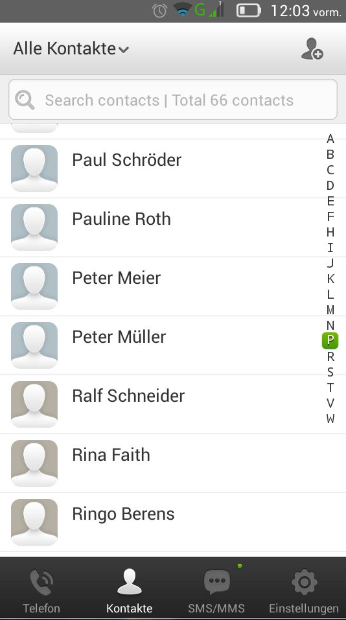
\includegraphics[scale=0.28]{peter}
	\label{Adressbuch} 
	\end{minipage}
% \caption{noch eine Caption}
\end{figure}
\pause
\begin{block}{Fokus}$\rightarrow$ 3 Disambiguierungstrategien untersucht \end{block} 
}



\section{Disambiguierungsstrategien}

\subsection{1. Disambiguierungsstrategie}
\frame{\frametitle{1. Disambiguierungsstrategie: \\Aggregierte Auswahl ohne Pause}

\begin{itemize}
\item alle möglichen Interpretationen in einer Sprachausgabe 
\item keine Pause zwischen Interpretationen
\item auf Auswahl des Benutzers gewartet
\end{itemize}

\begin{table}
\begin{tabular}{l|l }
\textbf{Akteur} &	\textbf{Sprachausgabe}\\
\hline \hline
Benutzer & Rufe Peter an!\\
System & Meinst du Peter Müller oder Peter Meier?\\
Benutzer & Peter Müller.\\
System & Ok, ich werde Peter Müller jetzt anrufen.\\
\end{tabular}
%\caption{Interaktionsbeispiel \texttt{Aggregierte Auswahl ohne Pause}}
\end{table}


}
\subsection{2. Disambiguierungsstrategie}
\frame{\frametitle{2. Disambiguierungsstrategie: \\Aggregierte Auswahl mit Pause}
\begin{itemize}
\item alle möglichen Interpretationen in einer Sprachausgabe 
\item Pause und Nummerierung zwischen Interpretationen
\item auf Auswahl des Benutzers gewartet
\end{itemize}

\begin{table}
\begin{tabular}{l|l }
\textbf{Akteur} &	\textbf{Sprachausgabe}\\
\hline \hline
Benutzer & Rufe Peter an!\\
System & Meinst du [Pause] 1. Peter Müller\\
& [Pause] oder 2. Peter Meier?\\
Benutzer & Erstens \\
System & Ok, ich werde Peter Müller jetzt anrufen.\\
\end{tabular}
%\caption{Interaktionsbeispiel \texttt{Aggregierte Auswahl ohne Pause}}
\end{table} 
}
\subsection{3. Disambiguierungsstrategie}
\frame{\frametitle{3. Disambiguierungsstrategie: \\Sequentielle Auswahl}
\begin{itemize}
\item alle möglichen Interpretationen in einer separaten Sprachausgabe 
\item auf Zustimmung/Ablehnung des Benutzer gewartet
\end{itemize}

\begin{table}
\begin{tabular}{l|l }
\textbf{Akteur} &	\textbf{Sprachausgabe}\\
\hline \hline
Benutzer & Rufe Peter an!\\
System & Meinst du Peter Meier?\\
Benutzer & Nein.\\
System & Meinst du Peter Müller?\\
Benutzer & Ja.\\
System & Ok, ich werde Peter Müller jetzt anrufen.\\
\end{tabular}
%\caption{Interaktionsbeispiel \texttt{Aggregierte Auswahl ohne Pause}}
\end{table} 
}

\section{Versuchsbeschreibung}
\subsection{Wizard-of-Oz}
\frame{\frametitle{Wizard-of-Oz}
\begin{itemize}
\item Die Existenz eines funktionierenden Systems wird vorgetäuscht
\newline
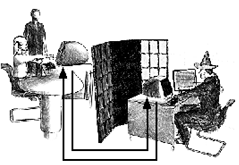
\includegraphics[scale=0.6]{woz}
\newline
\item Versuchspersonen wird der Eindruck verliehen, sie würde mit einem echten Dialogsystem interagieren
\item echtes Dialogsystem durch Versuchsleiter simuliert
\item Control Panel entwickelt, mit welchem Sprachausgaben ausgeben werden können
\end{itemize}
}

\subsection{Control Panel}
\frame{\frametitle{Control Panel}
\begin{figure}[h]
\caption{Control Panel}
	%\centering
        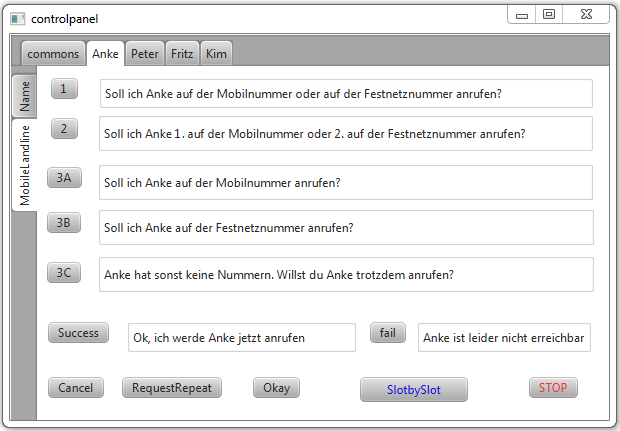
\includegraphics[scale=0.45]{controlpanel}
\end{figure}
}

\subsection{Testszenario}
\frame{\frametitle{Testszenario}
\begin{figure}[htbp]
	% minipage mit (Blind-)Text
	\begin{minipage}{0.60\textwidth} 
		\begin{itemize}
			\item Versuchspersonen sollen vorgegebenen Kontakt anrufen.
			\item Personenprofil zeigt Informationen über Kontakt
			\item unspezifische Spracheingabe: \newline $\rightarrow$ Disambiguierung
			\item pro Anruf unterschiedliche Disambiguierungstrategie
		\end{itemize}
	\end{minipage}
	\hfill
	\begin{minipage}{0.33\textwidth}
	\fbox{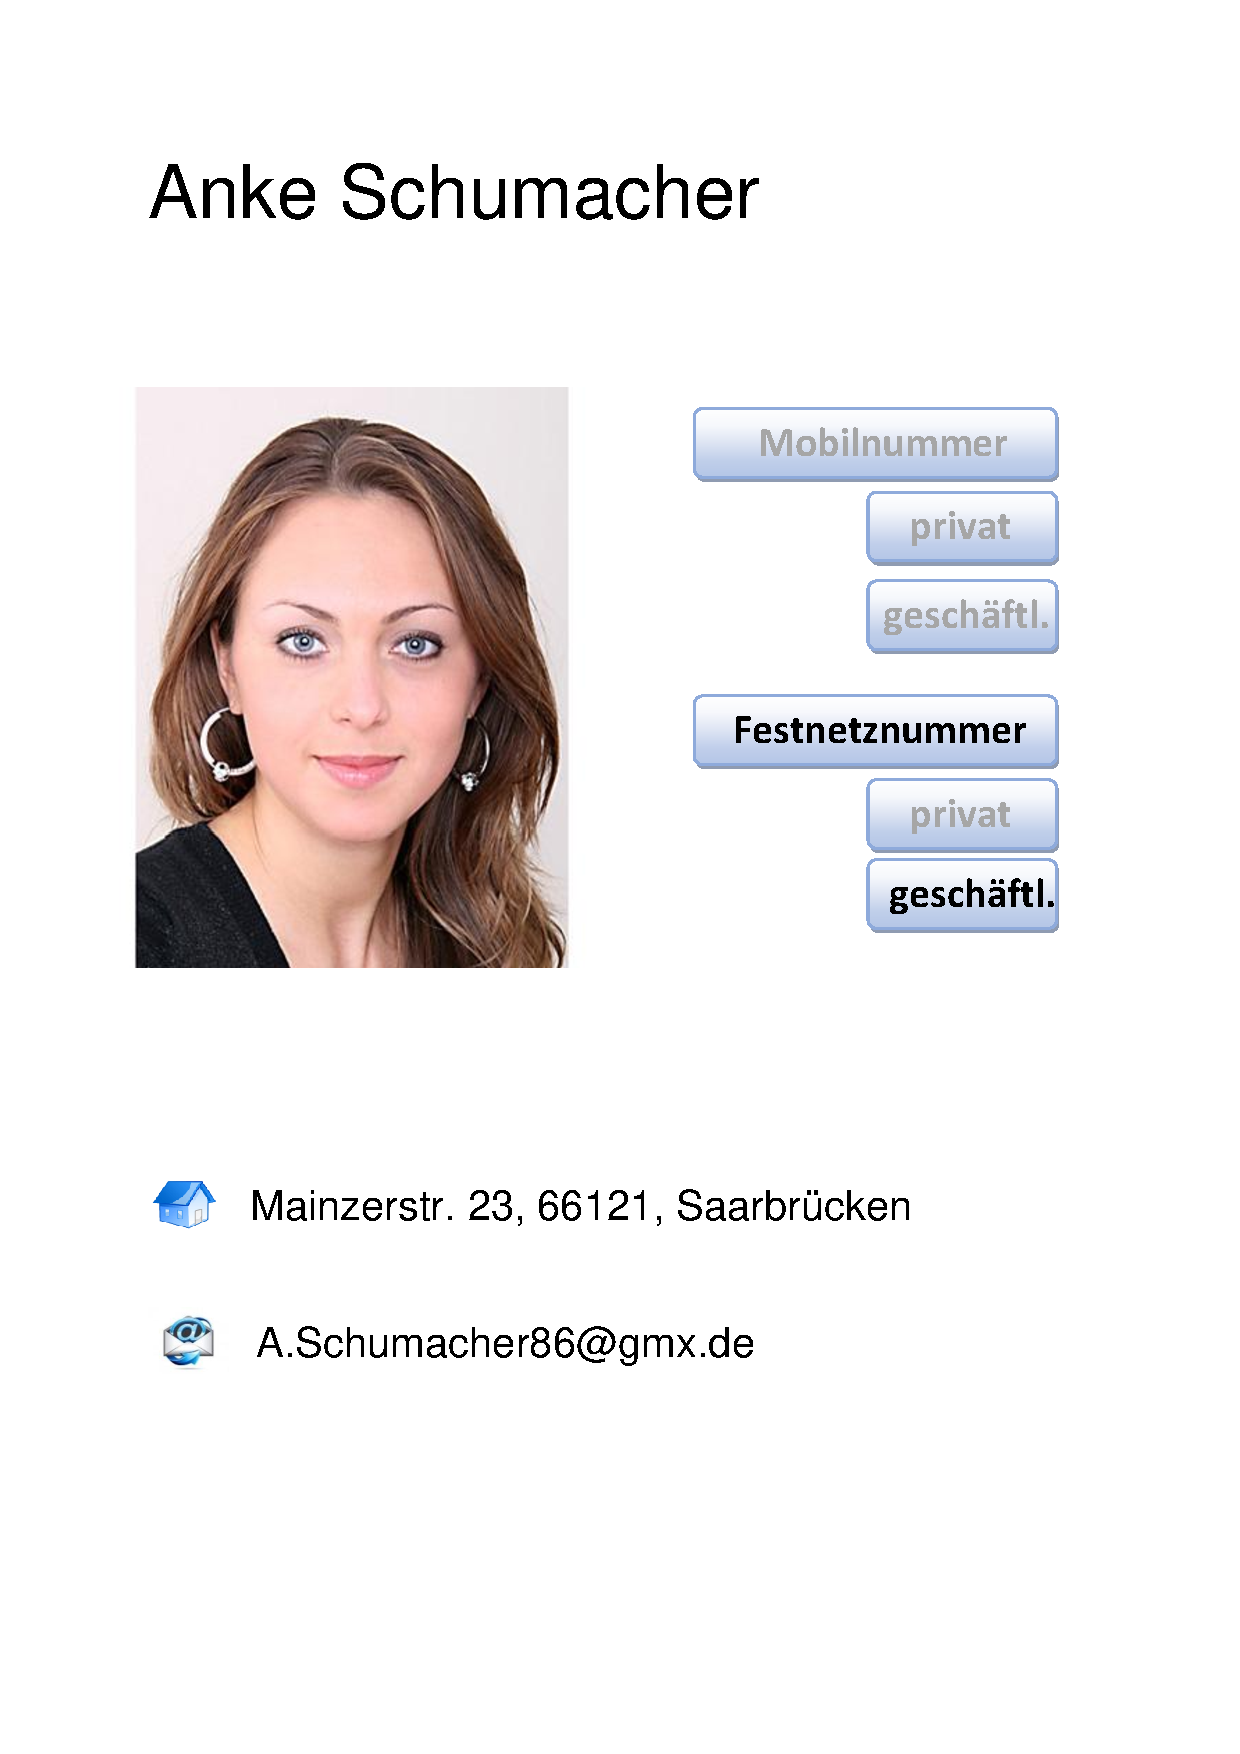
\includegraphics[scale=0.16]{Anke}}
	\label{Adressbuch} 
	\end{minipage}
% \caption{noch eine Caption}
\end{figure}
}
\subsection{Versuchsaufbau}

\frame{\frametitle{Versuchsaufbau}
\begin{itemize}
\item Versuchspersonen fahren ein Rennspiel. $\rightarrow$ Fahrsimulation
\item Rennspiel: Need for Speed: Shift
\item Rennspiel wird mit Lenkrad inklusive Gas- und Bremspedal gespielt  $\rightarrow$ realitätsgetreues Gefühl
\item Es wird im Einzelrennen mit jeweils 5 Gegnern gespielt
\item Versuchspersonen sollen möglichst hohe Platzierung erreichen \newline $\rightarrow$ Anstrengung und Konzentration soll hohe kognitive Belastung verursachen
\end{itemize} 
}

\frame{\frametitle{Versuchsaufbau - Rennspiel}
\begin{figure}[h]
\caption{Need for Speed - Shift}
	%\centering
        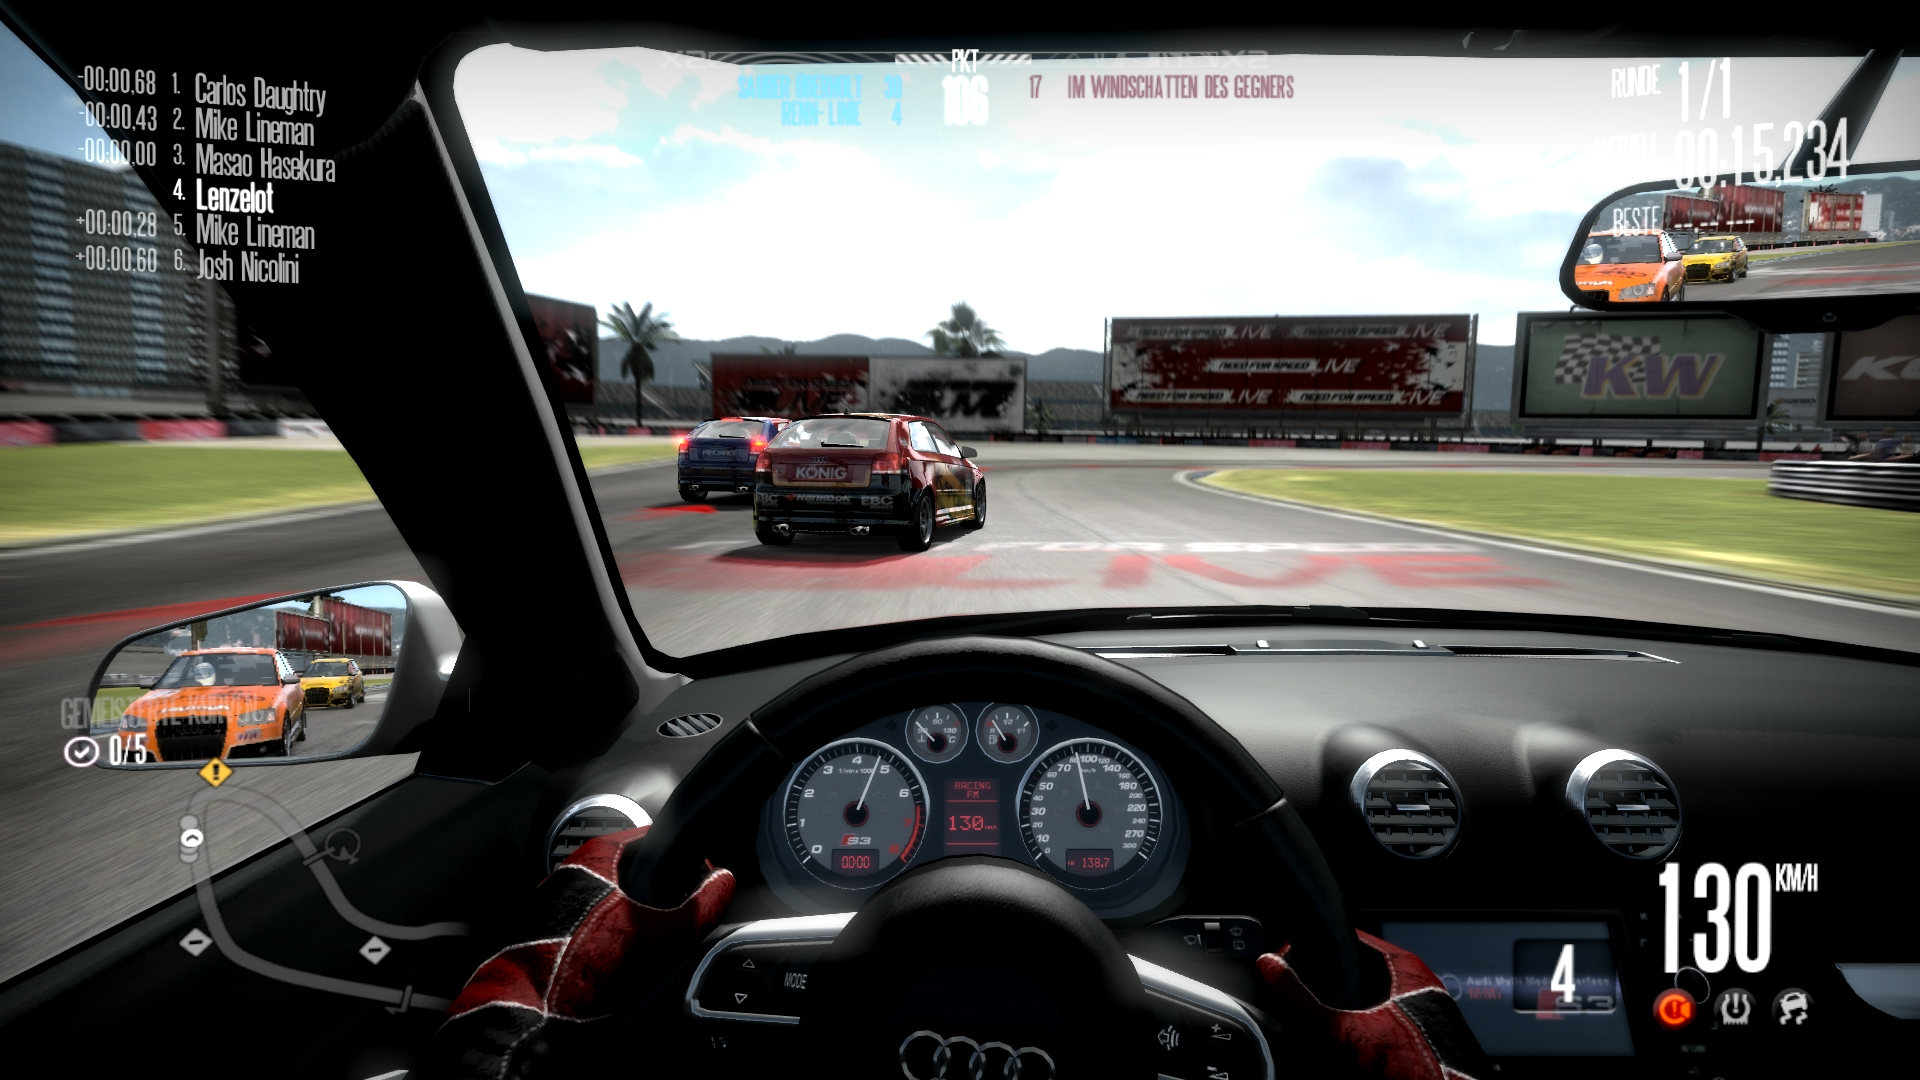
\includegraphics[scale=0.2]{nfs}
\end{figure}
}

\frame{\frametitle{Versuchsaufbau - Überblick}
\begin{table}
\begin{tabular}{l|l|l|l|l}
\textbf{Vorrunde}&\textbf{1. Runde}&\textbf{2. Runde} &\textbf{3. Runde} &\textbf{4. Runde}\\
\hline \hline
Rennspiel & Rennspiel & Rennspiel & Rennspiel &\\
 & Anruf Anke & Anruf Peter & Anruf Fritz & Anruf Kim \\
\end{tabular}
%\caption{Interaktionsbeispiel \texttt{Aggregierte Auswahl ohne Pause}}
\end{table}
\begin{itemize}
\item Vorrunde zum Einspielen
\item Runde 1-3: Rennspiel mit paralleler Systeminteraktion \newline $\rightarrow $ hohe kognitive Belastung
\item Runde 4: nur Systeminteraktion \newline $\rightarrow $ geringe kognitive Belastung
\end{itemize}
}

\frame{\frametitle{Versuchsdesign}
\begin{table}
\begin{tabular}{l|l|l|l}
\textbf{Aufteilung}&\textbf{Strecke 1}&\textbf{Strecke 2} &\textbf{Strecke 3}\\
\hline \hline
1. Gruppe & Strategie A & Strategie B & Strategie C \\
2. Gruppe & Strategie B & Strategie C & Strategie A\\
3. Gruppe  & Strategie C & Strategie A & Strategie B\\
4. Gruppe   & keine Strecke & keine Strecke & keine Strecke\\ 
\end{tabular}
%\caption{Interaktionsbeispiel \texttt{Aggregierte Auswahl ohne Pause}}
\end{table}
\begin{itemize}
\item 3 verschiedene Strecken, um Lerneffekt auszuschließen
\item jede Strecke mit unterschiedlicher Disambiguierungsstrategie
\item um Zeiten besser zu vergleichen: \newline $\rightarrow$ Disambiguierungsstrategien werden auf Strecken verteilt  \newline $\rightarrow$ Versuchspersonen werden in Gruppen (1-3) aufgeteilt
\item Die Strecken werden in gleicher Reihenfolge gefahren
\item Gruppe 4 führt das Testszenario mit zufälliger Strategie aus. 
\end{itemize}
}


\section{Versuch 1}
\subsection{Testszenario}
\frame{\frametitle{Testszenario}
\begin{figure}[htbp]
	% minipage mit (Blind-)Text
	\begin{minipage}{0.60\textwidth} 
		\begin{itemize}
			\item Testperson soll 4 Anrufe aufbauen
			\item Pro Anruf: Disambiguierung über zwei Merkmalen
			\item Disambiguierung erfolgt mit 2 Alternativen
			\item Personenprofil zeigt zu füllende Disambiguierungsmerkmale
		\end{itemize}
	\end{minipage}
	\hfill
	\begin{minipage}{0.30\textwidth}
	\fbox{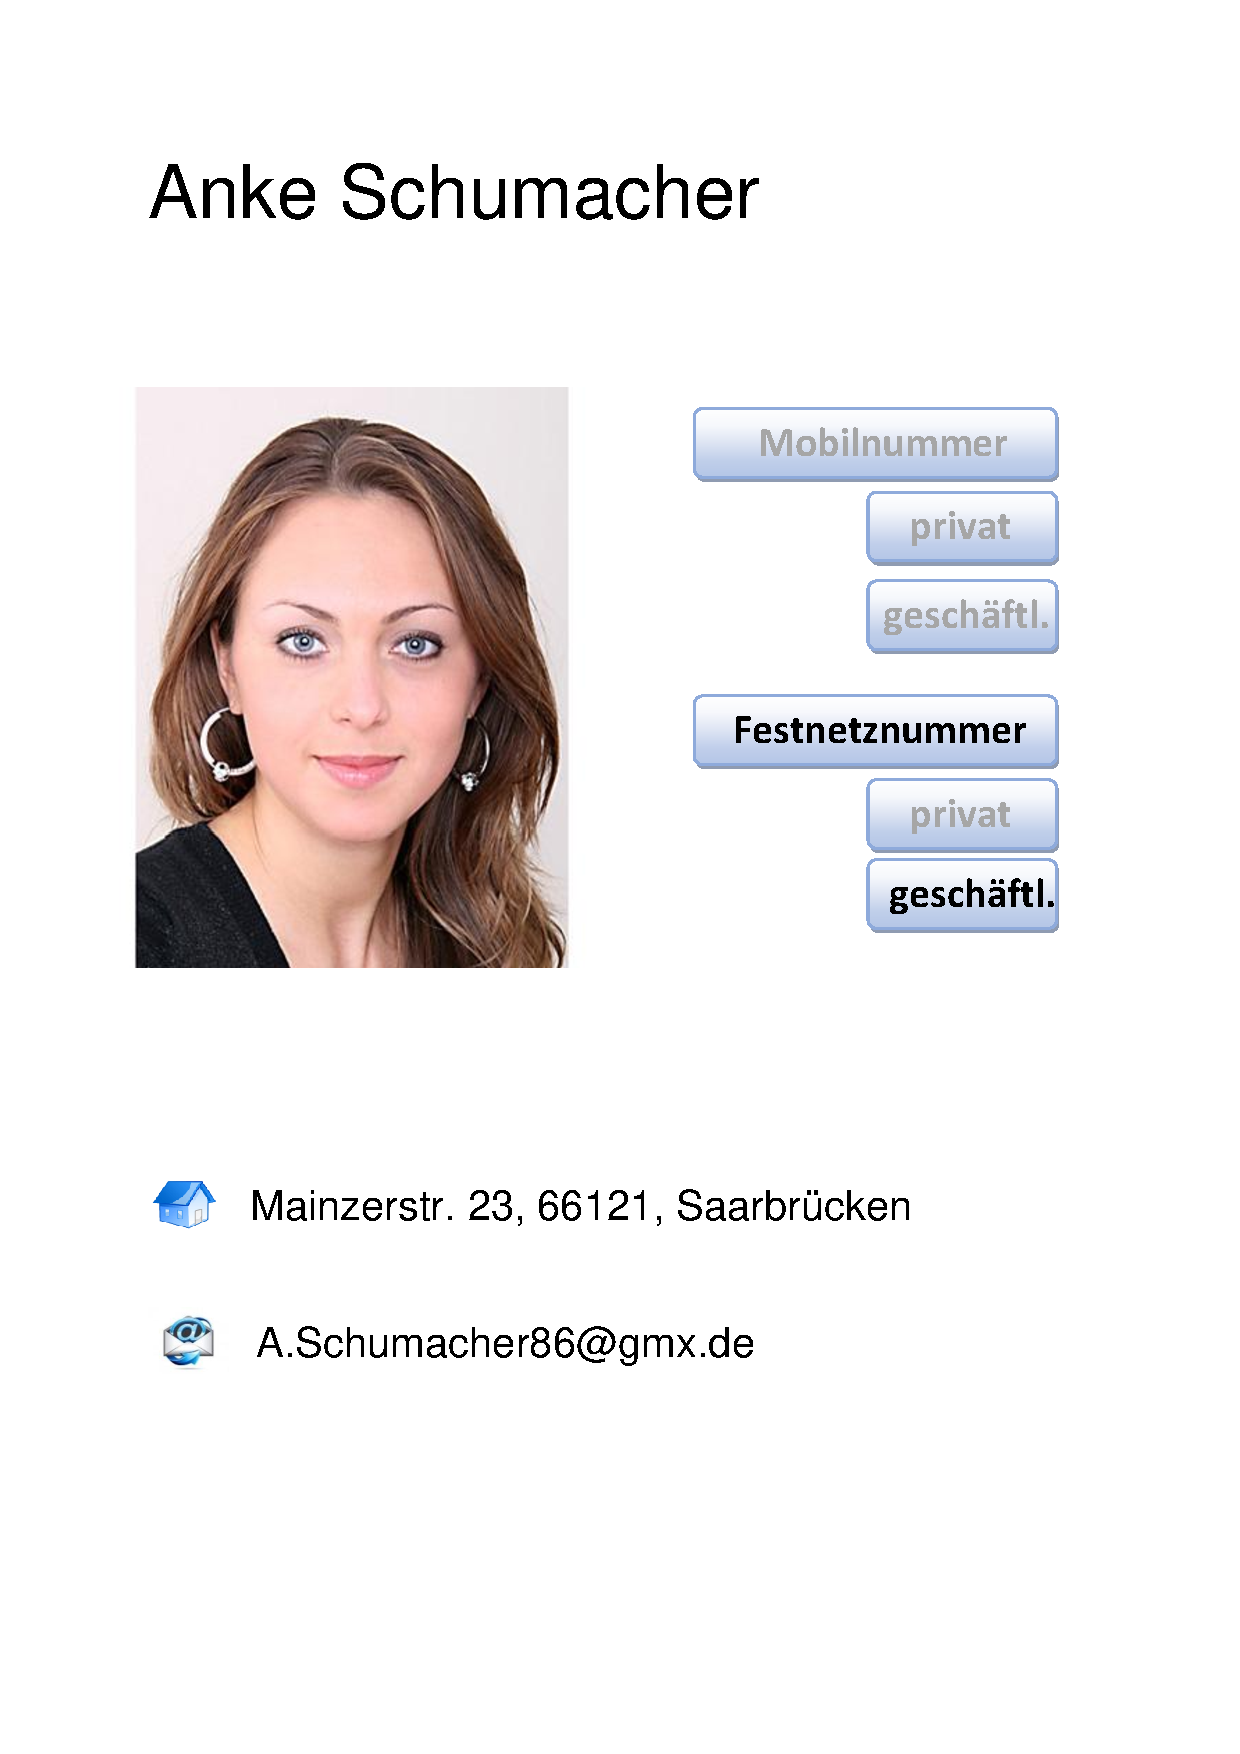
\includegraphics[scale=0.13]{Anke}}
	\label{Adressbuch} 
	\end{minipage}
% \caption{noch eine Caption}
\end{figure}
\begin{block}{Beispiel: Disambiguierung über Namen} Benutzer: Rufe Anke an \newline System:\quad Meinst du Anke Meier oder Schuhmacher? \newline Benutzer: Schuhmacher \end{block}
}
\subsection{Versuchspersonen}
\frame{\frametitle{Versuchspersonen}
\begin{itemize}
\item 12 deutsche Muttersprachler
\item 58\% 18-29 Jahre, 17\% 30-41 Jahre, 25\% 42-53 Jahre
\item 75\% keine bzw. wenig Erfahrung mit Dialogsystemen
\item 83\% spielen selten Rennspiele
\item 58\% fiel Einführungsrunde schwer
\end{itemize}

}

\subsection{Auswertung}
\frame{\frametitle{Auswertung}
Folgende Punkte werden ausgewertet
\newline
\begin{itemize}
\item Zeiten werden gemessen
	\begin{itemize}
		\item Rennzeiten
		\item Dialogzeiten
	\end{itemize}
\item Fragebögen ausgewertet
	\begin{itemize}
		\item Nasa-TLX
		\item Strategien
	\end{itemize}
\item Task Completion
\end{itemize} 
}

\frame{\frametitle{Gemessene Zeiten - Rennzeiten}
\begin{block}{Rennzeiten}Beeinflusst eine Disambiguierungsstrategie das Rennverhalten? \end{block} 
\begin{table}

\begin{tabular}{l|l|l|l}
\textbf{Rennzeiten}&\textbf{Strategie 1}&\textbf{Strategie 2} &\textbf{Strategie 3}\\
\hline \hline
Durchschnitt & \textcolor{blue}{71,58 sek} & 75,71 sek & \textcolor{red}{75,92 sek} \\
\end{tabular}
\end{table}
Zeiten statistisch nicht relevant und daher nicht aussagekräftig. 
}

\frame{\frametitle{Gemessene Zeiten - Dialogzeiten}
\begin{block}{Dialogzeiten}Welche Strategie ermöglicht den kürzesten Dialog? \end{block} 
Nur die Zeiten von korrekt durchgeführten Dialogen bewertet.
\begin{table}
\begin{tabular}{l|l|l|l}
\textbf{Dialogzeiten}&\textbf{Strategie 1}&\textbf{Strategie 2} &\textbf{Strategie 3}\\

\hline \hline
mit Rennspiel & \textcolor{blue}{15,2 sek} & \textcolor{red}{20,5 sek} & \textcolor{red}{20,8 sek} \\
ohne Rennspiel &   \textcolor{blue}{14,9 sek} &  \textcolor{red}{18,8 sek} &  \textcolor{red}{17,6 sek} \\
\end{tabular}
\end{table}  
$\rightarrow$ Strategie 1 ermöglicht den kürzesten Dialog. 
}
\frame{\frametitle{Gemessene Zeiten - Dialogzeiten}
\begin{block}{Rennzeiten}Gibt es Unterschiede in den Dialogzeiten zwischen kognitiv hoch belasteten und kognitiv wenig belasteten Versuchspersonen? \end{block} 
\begin{table}
\begin{tabular}{l|l|l|l}
\textbf{Dialogzeiten}&\textbf{Strategie 1}&\textbf{Strategie 2} &\textbf{Strategie 3}\\

\hline \hline
mit Rennspiel & \textcolor{red}{15,2 sek} & \textcolor{red}{20,5 sek} & \textcolor{red}{20,8 sek} \\
ohne Rennspiel &   \textcolor{blue}{14,9 sek} &  \textcolor{blue}{18,8 sek} &  \textcolor{blue}{17,6 sek} \\
\end{tabular}
\end{table} 
\begin{itemize}
\item kürzere Dialogzeiten ohne Rennspiel erreicht
\end{itemize}
$\rightarrow$ bessere Reaktionszeit bei Dialoginteraktion ohne Rennspiel
}

\frame{\frametitle{Fragebogen - Nasa-TLX}
\begin{block}{Nasa-TLX} 
\begin{enumerate}
\item  Bei welcher Stratgie wurde eine höhere Belastung empfunden?
\item  Gibt es Unterschiede in der Belastung zwischen den Runden mit und ohne Rennspiel?
\end{enumerate}
\end{block}

\begin{itemize}
\item geistige Anforderung
	\begin{itemize}
		\item Strategie 1: geringe geistige Anforderung
		\item Strategie 3: höchste geistige Anforderung
		\item Runde ohne Rennspiel weniger anfordernd
	\end{itemize}
\item Anstrengung
	\begin{itemize}
		\item Strategie 1: geringe Anstrengung
		\item Strategie 3: höchste Anstrengung
		\item Runde ohne Rennspiel weniger anstrengend
	\end{itemize}
\end{itemize}

$\rightarrow$ Stragie 1 am wenigsten belastend gewertet\newline


}

\frame{\frametitle{Fragebogen - Strategien}
\begin{block}{Strategien} Wie werden die Strategien von den Versuchspersonen bewertet? \end{block}


\begin{itemize}
\item Strategie 1 lenkte am wenigsten ab
\item Dialog aus Stratgie 1 gefiel am besten, Strategie 3 am schlechtesten
\item Strategie 1 wurde von 75\% als beste Strategie gewählt \newline(17\% Strategie 2, 8\% Strategie 1) \newline
\item der Dialog fiel im Durchschnitt ohne Rennspiel einfacher \newline
\end{itemize}
$\rightarrow$ Strategie 1 insgesamt am besten bewertet
\newline
}



\frame{\frametitle{Task Completion}
\begin{block}{Task Completion (TC)} Welche Strategie ist am erfolgversprechendsten? \end{block}
\begin{itemize}
\item Die Task Completion wird für jeden Dialog wie folgt berechnet:
	\begin{itemize}
	\item 0 Punkte, wenn kein Slot richtig gefüllt wird
	\item 1 Punkt, wenn ein Slot richtig gefüllt wird
	\item 2 Punkte, wenn alle Slots richtig gefüllt werden
	\end{itemize}
\item für jede Strategie wird die durchschnittliche Task Completion bewertet
\end{itemize}
}

\frame{\frametitle{Task Completion}
%\begin{block}{Task Completion (TC)} Welche Strategie ist am erfolgversprechendsten? \end{block}

\begin{table}
\begin{tabular}{l|l|l|l}

\textbf{Strategien}&\textbf{Runde 1-4}&\textbf{Runde 1-3} &\textbf{Runde 4}\\
	\hline \hline
1. Strategie & 1,75 & 1,92 & 1,50  \\
2. Strategie & \textcolor{blue}{1,94} & 1,92 & 2,00  \\
3. Strategie & \textcolor{red}{1,63} & 1,50 & 2,00  \\
\hdashline
alle Strategien & & \textcolor{red}{1,78} & \textcolor{blue}{1,83} \\ 
\end{tabular}
\end{table}

\begin{itemize}
\item Strategie 2 am erfolgreichsten
\item Strategie 3 am unerfolgreichsten 
\newline
\item Runde ohne Rennspiel erfolgreicher als Runden mit Rennspiel
\newline
\end{itemize}
$\rightarrow$ Unterschied gering: Mehr Werte benötigt 
}


\frame{\frametitle{Auswertung - Zusammenfassung}
\begin{itemize}
\item \textbf{kürzeste Rennzeit}: nicht aussagekräftig
\item \textbf{kürzeste Dialogzeit}: Strategie 1
\item Ergebnis \textbf{Nasa-TLX} Fragebogen:
	\begin{itemize}
		\item Strategie 1 am unbelastetsten
		\item Runde ohne Rennspiel weniger belastend als Runde mit
	\end{itemize}
\item Ergebnis \textbf{Strategien} Fragebogen:
	\begin{itemize}
		\item Strategie 1 am positivsten bewertet
		\item Dialog fiel im Durchschnitt ohne Rennspiel einfacher
	\end{itemize}
\item \textbf{Task Completion} 
	\begin{itemize}
		\item Strategie 2 > Strategie 1 > Strategie 3 (geringer Unterschied)
		\item Dialog ohne Rennspiel erfolgreicher als Dialog ohne Rennspiel
	\end{itemize}
\end{itemize}
$\Rightarrow$ \textcolor{blue}{Strategie 1} am Effizientesten und Beliebtesten
}

\section{Versuch 2}

\subsection{Versuchsbeschreibung}
\frame{\frametitle{Versuch 2}
Versuch 1 zeigte eindeutiges Ergebnis bei Disambiguierung über 2 Alternativen \newline
\begin{block}{Fragestellung}Gleiches Ergebnis bei Disambiguierung über mehr Alternativen? \end{block} 
\begin{itemize}
\item[$\rightarrow$] Zweiter Versuch eingeleitet:
\begin{itemize}
\item gleiche Versuchsdurchführung
\item Unterschied zu Versuch 1: längere Disambiguierung
\end{itemize}
\end{itemize}
}



\subsection{Testszenario}
\frame{\frametitle{Testszenario}
\begin{figure}[htbp]
	% minipage mit (Blind-)Text
	\begin{minipage}{0.60\textwidth} 
		\begin{itemize}
			\item Testperson soll 4 Anrufe aufbauen
			\item Pro Anruf: Disambiguierung über zwei Merkmalen
			\item Disambiguierung erfolgt mit 6 Alternativen
			\item Personenprofil zeigt zu füllende Disambiguierungsmerkmale
		\end{itemize}
	\end{minipage}
	\hfill
	\begin{minipage}{0.30\textwidth}
	\fbox{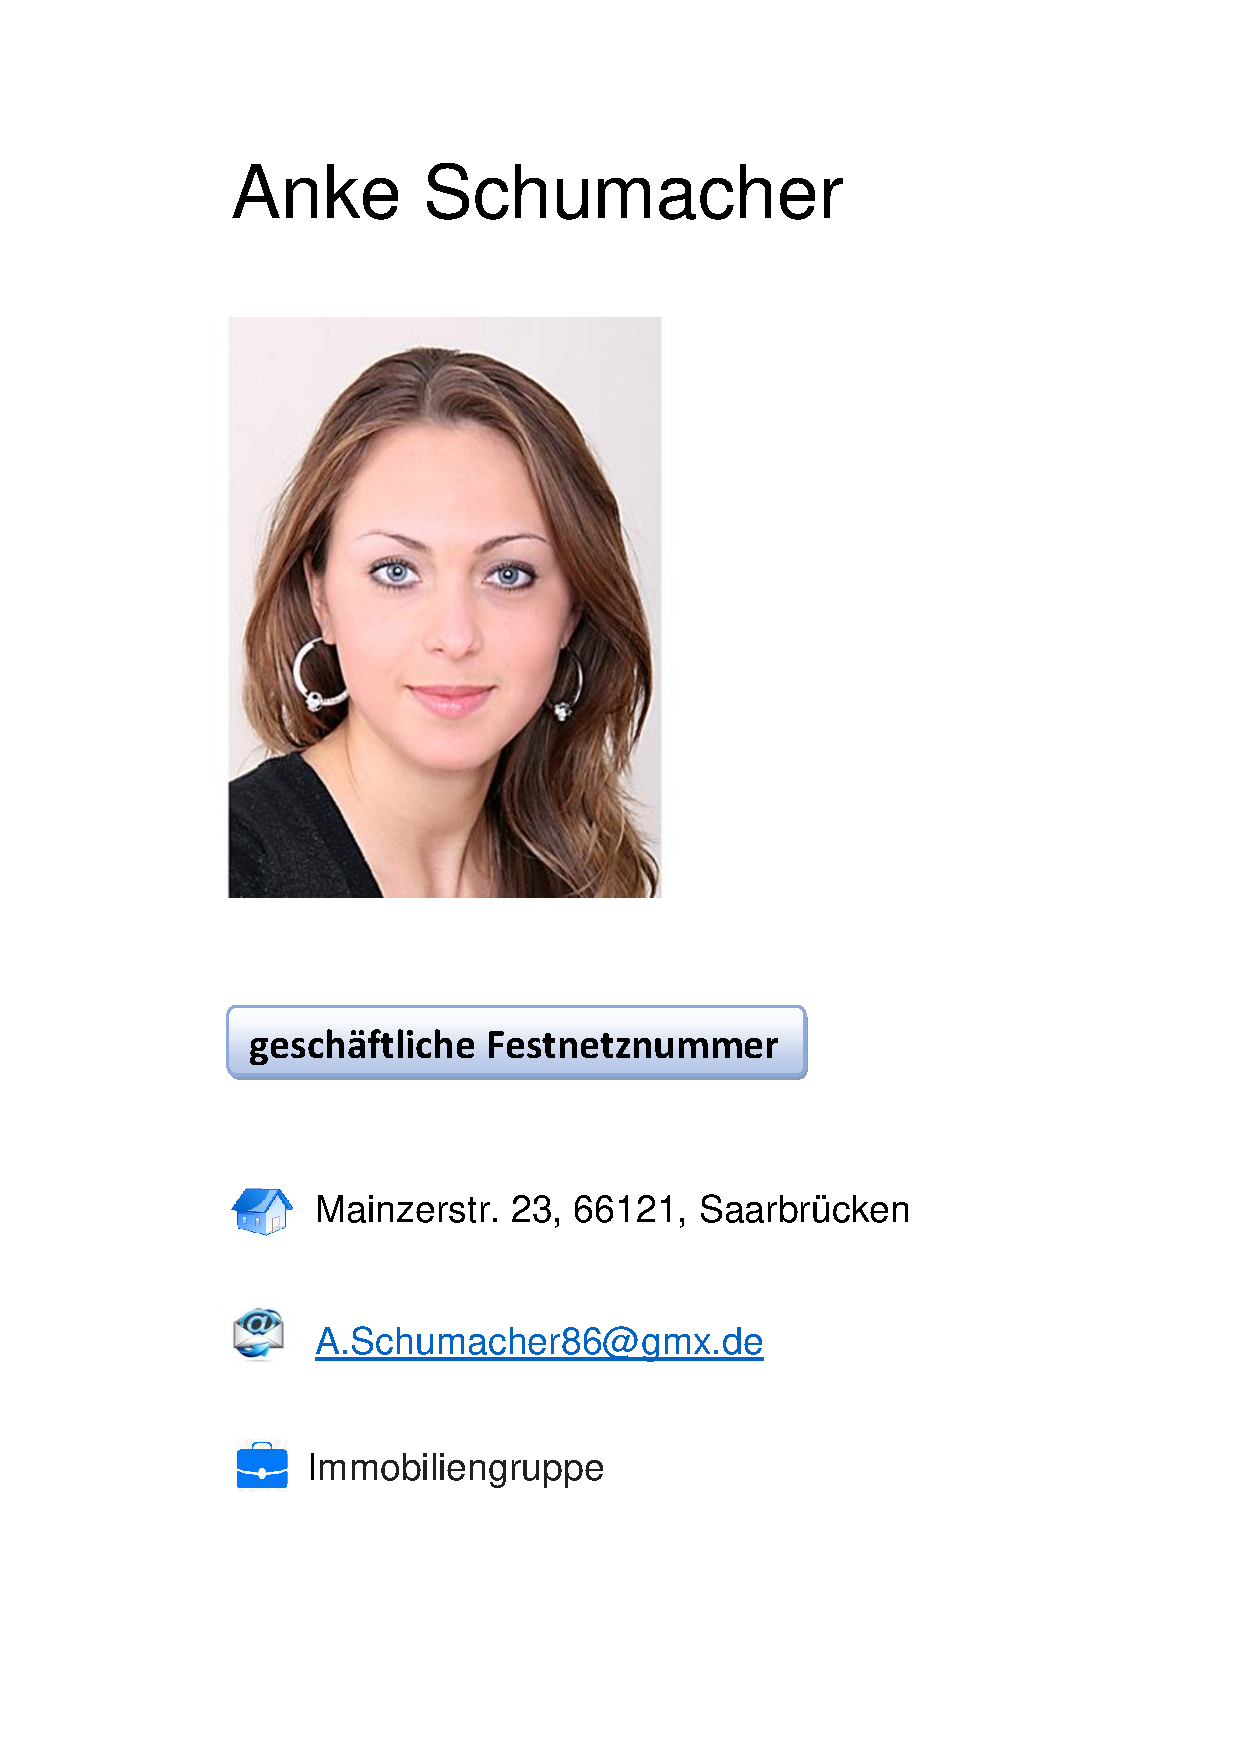
\includegraphics[scale=0.11]{Anke2}}
	\label{Adressbuch} 
	\end{minipage}
% \caption{noch eine Caption}
\end{figure}
\begin{block}{Beispiel: Disambiguierung über Namen} Benutzer: Rufe Anke an \newline System:\quad Meinst du Anke Bies, Anke Elb, ... oder Anke Weiler? \newline Benutzer: Schuhmacher \end{block}
}

\subsection{Versuchspersonen}
\frame{\frametitle{Versuchspersonen}
\begin{itemize}
\item 12 deutsche Muttersprachler
\item 42\% 18-29 Jahre, 25\% 30-41 Jahre, 33\% 42-53 Jahre
\item 75\% keine bzw. wenig Erfahrung mit Dialogsystemen
\item 83\% spielen selten Rennspiele
\item 58\% fiel Einführungsrunde schwer \newline
\item[$\rightarrow$] Zufällig gleiche Erfahrungswerte wie in Versuch 1: \newline
\item[$\rightarrow$]  Unterschiedliche Resultate der Versuche nicht durch unterschiedliche Erfahrung zu erklären

\end{itemize}


}

\subsection{Auswertung}
\frame{\frametitle{Auswertung}
Folgende Punkte werden ausgewertet
\newline
\begin{itemize}
\item Zeiten werden gemessen
	\begin{itemize}
		\item Rennzeiten
		\item Dialogzeiten
	\end{itemize}
\item Fragebögen ausgewertet
	\begin{itemize}
		\item Nasa-TLX
		\item Strategien
	\end{itemize}
\item Task Completion
\end{itemize} 
}

\frame{\frametitle{Gemessene Zeiten - Rennzeiten}
\begin{block}{Rennzeiten}Beeinflusst eine Disambiguierungsstrategie das Rennverhalten? \end{block} 
\begin{table}

\begin{tabular}{l|l|l|l}
\textbf{Rennzeiten}&\textbf{Strategie 1}&\textbf{Strategie 2} &\textbf{Strategie 3}\\
\hline \hline
Durchschnitt & {76,83 sek} & \textcolor{red}{77,47 sek} & \textcolor{blue}{76,73 sek} \\
\end{tabular}
\end{table}
Zeiten statistisch nicht relevant und daher nicht aussagekräftig. 
}

\frame{\frametitle{Gemessene Zeiten - Dialogzeiten}
\begin{block}{Dialogzeiten}Welche Strategie ermöglicht den kürzesten Dialog? \end{block} 
Nur die Zeiten von korrekt durchgeführten Dialogen bewertet.
\begin{table}
\begin{tabular}{l|l|l|l}
\textbf{Dialogzeiten}&\textbf{Strategie 1}&\textbf{Strategie 2} &\textbf{Strategie 3}\\

\hline \hline
mit Rennspiel & \textcolor{blue}{29,6 sek} & \textcolor{red}{38,5 sek} & \textcolor{red}{34,3 sek} \\
ohne Rennspiel &   \textcolor{blue}{24,1 sek} &  \textcolor{red}{34,4 sek} &  \textcolor{red}{30,4 sek} \\
\end{tabular}
\end{table}  
$\rightarrow$ Strategie 1 ermöglicht den kürzesten Dialog. 
}
\frame{\frametitle{Gemessene Zeiten - Dialogzeiten}
\begin{block}{Rennzeiten}Gibt es Unterschiede in den Dialogzeiten zwischen kognitiv hoch belasteten und kognitiv wenig belasteten Versuchspersonen? \end{block} 
\begin{table}
\begin{tabular}{l|l|l|l}
\textbf{Dialogzeiten}&\textbf{Strategie 1}&\textbf{Strategie 2} &\textbf{Strategie 3}\\

\hline \hline
mit Rennspiel & \textcolor{red}{29,6 sek} & \textcolor{red}{38,5 sek} & \textcolor{red}{34,3 sek} \\
ohne Rennspiel &   \textcolor{blue}{24,1 sek} &  \textcolor{blue}{34,4 sek} &  \textcolor{blue}{30,4 sek} \\
\end{tabular}
\end{table} 
\begin{itemize}
\item kürzere Dialogzeiten ohne Rennspiel erreicht
\end{itemize}
$\rightarrow$ bessere Reaktionszeit bei Dialoginteraktion ohne Rennspiel 
}

\frame{\frametitle{Fragebogen - Nasa-TLX}
\begin{block}{Nasa-TLX} 
\begin{enumerate}
\item  Bei welcher Stratgie wurde eine höhere Belastung empfunden?
\item  Gibt es Unterschiede in der Belastung zwischen den Runden mit und ohne Rennspiel?
\end{enumerate}
\end{block}

\begin{itemize}
\item geistige Anforderung
	\begin{itemize}
		\item Strategie 3: höchste geistige Anforderung
		\item Runde ohne Rennspiel weniger anfordernd
	\end{itemize}
\item Anstrengung
	\begin{itemize}
		\item Strategie 3: geringe Anstrengung
		\item Strategie 2: höchste Anstrengung
		\item Runde ohne Rennspiel weniger anstrengend
	\end{itemize}
\end{itemize}

$\rightarrow$ Unterschiedliche empfundene Belastung mit und ohne Rennspiel \newline
$\rightarrow$ keine Aussage über belastendste Strategie treffbar.


}

\frame{\frametitle{Fragebogen - Strategien}
\begin{block}{Strategien} Wie werden die Strategien von den Versuchspersonen bewertet? \end{block}


\begin{itemize}
\item Strategie 2 lenkte am wenigsten ab, Strategie 1 am meisten
\item Dialog aus Stratgie 3 gefiel am besten
\item Strategie 3 wurde von 50\% als beste Strategie gewählt \newline (17\% Strategie 1, 33\% Strategie 2) \newline
\item der Dialog fiel im Durchschnitt ohne Rennspiel einfacher\newline
\end{itemize}
$\rightarrow$ keine Strategie eindeutig am besten bewertet \newline
$\rightarrow$ Strategie 3 am beliebtesten bewertet

}



\frame{\frametitle{Task Completion}
\begin{block}{Task Completion (TC)} Welche Strategie ist am erfolgversprechendsten? \end{block}
\begin{itemize}
\item Die Task Completion wird für jeden Dialog wie folgt berechnet:
	\begin{itemize}
	\item 0 Punkte, wenn kein Slot richtig gefüllt wird
	\item 1 Punkt, wenn ein Slot richtig gefüllt wird
	\item 2 Punkte, wenn alle Slots richtig gefüllt werden
	\end{itemize}
\item für jede Strategie wird die durchschnittliche Task Completion bewertet
\end{itemize}
}

\frame{\frametitle{Task Completion}
%\begin{block}{Task Completion (TC)} Welche Strategie ist am erfolgversprechendsten? \end{block}

\begin{table}
\begin{tabular}{l|l|l|l}

\textbf{Strategien}&\textbf{Runde 1-4}&\textbf{Runde 1-3} &\textbf{Runde 4}\\
	\hline \hline
1. Strategie &  \textcolor{blue}{1,88} & 1,83 & 2,00  \\
2. Strategie & 1,81 & 1,75 & 2,00  \\
3. Strategie & \textcolor{red}{1,56} & 1,42 & 2,00  \\
\hdashline
alle Strategien & & \textcolor{red}{1,67} & \textcolor{blue}{2,00} \\ 
\end{tabular}
\end{table}

\begin{itemize}
\item Strategie 1 am erfolgreichsten
\item Strategie 3 am unerfolgreichsten 
\newline
\item Runde ohne Rennspiel erfolgreicher als Runden mit Rennspiel
\newline
\end{itemize}
$\rightarrow$ Unterschied gering: Mehr Werte benötigt 
}


\frame{\frametitle{Auswertung - Zusammenfassung}
\begin{itemize}
\item \textbf{kürzeste Rennzeit}: nicht aussagekräftig
\item \textbf{kürzeste Dialogzeit}: Strategie 1
\item Ergebnis \textbf{Nasa-TLX} Fragebogen:
	\begin{itemize}
		\item kein eindeutiges Ergebnis über belastendste Strategie
		\item Runde ohne Rennspiel weniger belastend als Runde mit
	\end{itemize}
\item Ergebnis \textbf{Strategien} Fragebogen:
	\begin{itemize}
		\item keine Strategie eindeutig am besten bewertet
		\item Strategie 3 am beliebtesten
		\item Dialog fiel im Durchschnitt ohne Rennspiel einfacher
	\end{itemize}
\item \textbf{Task Completion} 
	\begin{itemize}
		\item Strategie 1 > Strategie 2 > Strategie 3 (geringer Unterschied)
		\item Dialog ohne Rennspiel erfolgreicher als Dialog ohne Rennspiel
	\end{itemize}
\end{itemize}
$\Rightarrow$ \textcolor{blue}{Strategie 1} am Effizientesten \newline
$\Rightarrow$ \textcolor{blue}{Strategie 3} am Beliebtesten


}



\section{Ergebnis}

\frame{\frametitle{Auswertung - Zusammenfassung}
\begin{block}{Erkenntnis}Länge der Disambiguierung beeinflusst Strategienbeliebtheit bzw. Strategieneffizienz \end{block}

\begin{itemize}
\item Disambiguierung $\le$ 2 Alternativen: 
	\begin{itemize}
	\item[$\Rightarrow$] Strategie 1 beliebt und effizient
	\end{itemize}
\item Disambiguierung $\ge$ 2 Alternativen:
	\begin{itemize}
	\item[$\Rightarrow$] Strategie 1 effizient
	\item[$\Rightarrow$] Strategie 3 beliebt
	\end{itemize}
\end{itemize}

}





\end{document}

